\section{Margin-aware diagnostics and a directional-loss confirmation}

This follow-up was specified after the preceding experiments. Old-model diagnostics motivate a new-source, new-test intervention; they are not independent confirmation.

With row-vector conventions and first-step error $e$, the output change induced by its readout-nullspace part is $d_{\mathrm{null}}=eQ M_B W^\top$, where $Q$ projects onto $\ker W$. This preserves all first-step numeric logits, not every possible nonlinear answer code. We compare harmful rival-score shifts with the corresponding true-intermediate classification margins. Oracle-correct inputs are analyzed separately.

At equal perturbation norm (10\% of centered intermediate hidden RMS), old matrix-model collision accuracy falls from 99.2\% to 53.6\% in the actual null-error direction; the corresponding permutation figures are 93.3\% and 92.3\%. Random null directions are also tested at identical norm. The analysis is conditional on old trained models and test distributions and does not establish a universal domain ordering.

\begin{figure}[h]\centering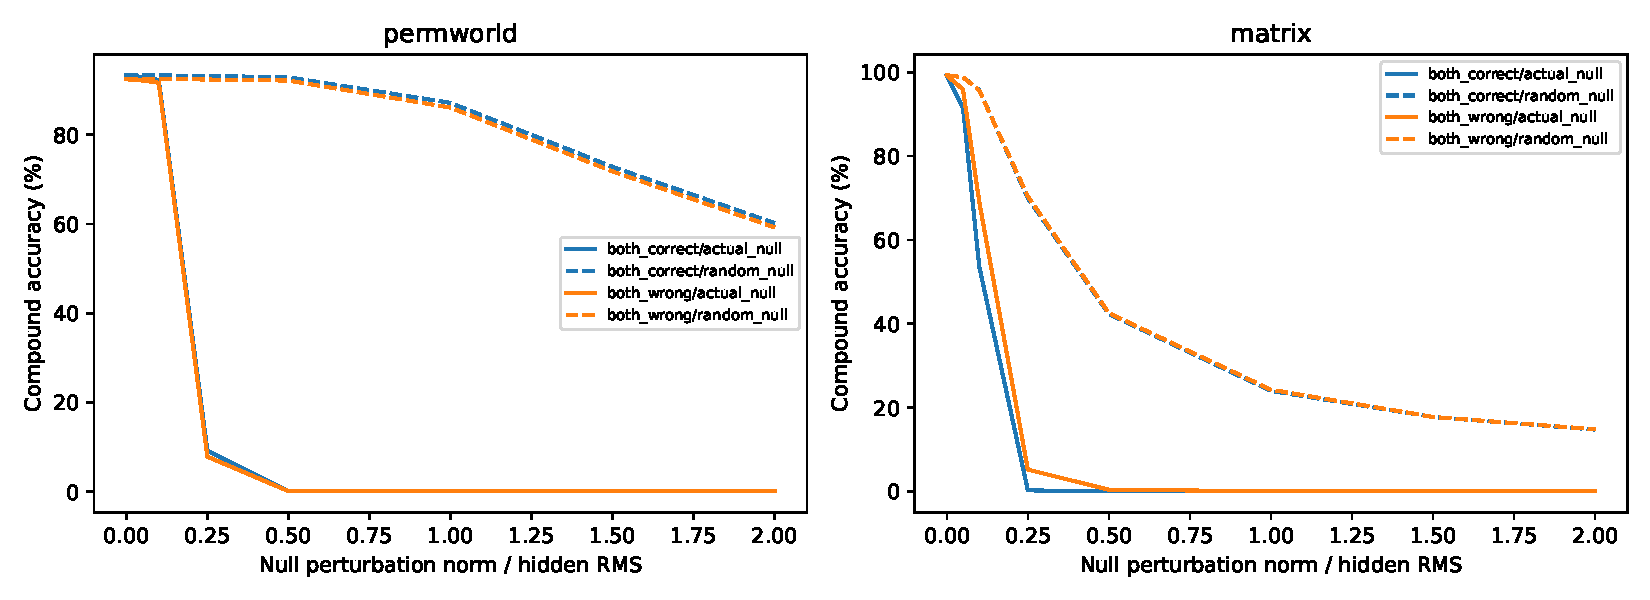
\includegraphics[width=\linewidth]{../results/downstream_harm_diagnostic_v2/perturbations.pdf}

\caption{Equal-norm actual-error and random-null perturbations of true intermediate states. Real intermediates are diagnostic information, not inputs available to the deployed predictor.}\end{figure}

\paragraph{Predictor capacity diagnostic.} We fit an affine residual and a one-hidden-layer GELU residual on only base-to-first-generator training states, using 2000 fixed updates and a frozen second operator and readout. Neither compound targets nor compound labels enter fitting. The nonlinear residual has approximately four times as many trainable parameters as the affine residual; this is not a capacity-matched comparison.

\begin{center}\begin{tabular}{llrr}\toprule Domain & First predictor & Compound (\%) & Both correct (\%)\\\midrule
matrix & Original affine & 9.64 & 0.00\\
matrix & Affine residual & 9.64 & 0.78\\
matrix & Nonlinear residual & 50.65 & 25.78\\
permworld & Original affine & 35.89 & 10.42\\
permworld & Affine residual & 38.75 & 13.18\\
permworld & Nonlinear residual & 45.62 & 20.05\\
\bottomrule\end{tabular}\end{center}

The capacity diagnostic uses three old source models per domain. Without matched-wrong nonlinear targets it cannot identify the causal effect of mathematical correctness. Identical-budget replay saves all predictors and forecasts and independently reproduces the initial diagnostic without tuning.

\paragraph{Prospective loss-direction intervention.} Each domain uses three new ordinary-source initializations and one fresh support pool per source. Full versus null-only geometric objectives are crossed with correct versus answer-matched wrong pairings. Each objective is normalized by the fixed ordinary teacher variance in its own space, using training states only. Native labels, teacher outputs, schedules, frozen readout, and all training budgets remain identical across the four arms. Permutation models train 20 epochs from initialization (distinct from the earlier dependent 10-to-20 continuation), and matrix models train 900 epochs. All twelve fits complete before the domain compound test opens.

Permutation sources reuse the original known-state corpus, so the new-source claim concerns initialization rather than new corpora. Their support and test orbits are excluded from all local archived input datasets. Matrix partitions are newly sampled, exclude previously examined matrix test orbits, and separate entire source/validation/support/test group orbits. Historical training orbits may recur under entirely new models.

\begin{center}\begin{tabular}{llrr}\toprule Domain & Direction/pairing & Compound (\%) & Both correct (\%)\\\midrule
matrix & full correct & 7.55 & 0.26\\
matrix & full wrong & 6.12 & 0.26\\
matrix & null correct & 9.64 & 0.78\\
matrix & null wrong & 9.51 & 0.78\\
permworld & full correct & 36.35 & 12.66\\
permworld & full wrong & 32.89 & 7.03\\
permworld & null correct & 12.55 & 0.21\\
permworld & null wrong & 14.66 & 0.42\\
\bottomrule\end{tabular}\end{center}

The predeclared primary statistic is the matrix accuracy interaction: $(\mathrm{null,correct}-\mathrm{null,wrong})-(\mathrm{full,correct}-\mathrm{full,wrong})$. Confidence intervals resample three source clusters and complete collision pairs. They do not treat the twelve models as twelve independent sources.

\begin{center}\begin{tabular}{lrr}\toprule Domain & Interaction (pp) & Source+pair 95\% interval\\\midrule
matrix & -1.30 & [-5.08, +2.60]\\
permworld & -5.57 & [-10.31, -1.46]\\
\bottomrule\end{tabular}\end{center}

Null-only loss removes the full-space row penalty as well as emphasizing null directions. In the new matrix study it lowers null error but permits larger readout-row state error; high primitive classification scores do not bound that error. Thus this experiment tests the specified replacement objective, not a scheme that retains the full-space term and adds null weighting.

No compound-outcome tuning or checkpoint selection was performed. A missing shared KD import was caught by a toy loss test and corrected before any permutation intervention fit; the initial script and pre-fit implementation amendment are retained. An initial diagnostic self-class division produced nonfinite margin statistics; the corrected implementation and independent rival-loop verification are preserved. The perturbation curves were unaffected.
